\section{Experiments}
\label{sec:experiments}

\subsection{Setup}

\paragraph{Benchmark.}
Real street panoramas with dense metric ground truth are not available to us at the time of writing
(\cref{sec:limitations}). We therefore use procedural street canyons with exact depth: a ground plane,
two building fa\c{c}ades 5--9\,m from the camera with random heights, end walls 60--120\,m away,
3--7 box-shaped parked vehicles, and sky. All surfaces carry a view-independent multi-scale procedural
texture. The reference panorama is at the origin and the partner $b$ metres further along the street,
the hardest configuration, because the epipoles look down the street. Unless stated otherwise,
panoramas are $256\times512$ and $b=4$\,m. The monocular prior is simulated as the true log-depth plus
spatially smooth noise with 6\% standard deviation and a global scale error drawn uniformly in
$\pm10\%$, with a constant self-reported $\sigma_p=0.06$; this matches the reported accuracy of current
panoramic foundation models~\cite{lin2026dap}. Calibration uses six scenes (seeds $\geq1000$), disjoint
from the ten test scenes, with ground truth standing in for the city teacher.

\paragraph{Baselines.}
All fusion variants share the same stereo, prior, scale alignment and gate, and differ only in the
stereo uncertainty $\sigma_s$:
\emph{constant} ($\sigma_s=s$) and \emph{confidence} ($\sigma_s=s/c$), with $s$ fitted on the same
calibration rays and with the same robust estimator as ours; \emph{selection}, which takes per ray the
source with the smaller calibrated $\sigma$; and our closed form without calibration
($\sigma_\theta=0.5$\,px). We also report the prior alone, the scale-aligned prior and stereo alone.

\paragraph{Metrics.}
Median relative depth error overall and per bin of the angle between ray and baseline; the fraction
of rays within 20\,cm; the fraction of errors within the predicted $1\sigma$ (ideal 0.683); the Gaussian
negative log-likelihood (NLL) in log-depth, a proper scoring rule for the predicted distribution;
and the area under the sparsification error curve (AUSE)~\cite{ilg2018uncertainty}.

\subsection{Main results}

\begin{table*}[t]
  \centering
  \resizebox{\linewidth}{!}{\begin{tabular}{l ccccc c ccc}
\toprule
 & \multicolumn{5}{c}{Median rel.\ error (\%) $\downarrow$, by angle to baseline} & $<$20\,cm (\%) $\uparrow$ & Cal.\ $1\sigma$ & NLL $\downarrow$ & AUSE $\downarrow$ \\
\cmidrule(lr){2-6}
Method & 0--10$^\circ$ & 10--30$^\circ$ & 30--60$^\circ$ & 60--90$^\circ$ & all & all & (0.68) & all & all \\
\midrule
Prior only & 6.81 & 7.04 & 6.99 & 6.92 & 6.95 & 29.80 & 0.44 & -0.73 & 0.481 \\
Prior + scale alignment & 4.45 & 4.03 & 3.83 & 3.98 & 3.94 & 47.12 & 0.69 & -1.40 & 0.534 \\
Stereo only & 21.07 & 3.03 & 2.05 & 1.49 & 1.78 & 68.99 & \textbf{0.68} & 26.04 & 0.386 \\
\midrule
Fusion, constant $\sigma_s$ & 4.90 & 2.41 & 1.76 & 1.48 & 1.64 & 73.66 & 0.73 & -2.17 & \textbf{0.329} \\
Fusion, confidence $\sigma_s$ & 4.49 & \textbf{2.35} & \textbf{1.73} & 1.43 & \textbf{1.60} & \textbf{74.10} & 0.73 & \textbf{-2.22} & 0.331 \\
Selection (min.\ $\sigma$) & 4.45 & 3.07 & 2.03 & 1.47 & 1.74 & 70.60 & 0.70 & -2.03 & 0.354 \\
Ours, closed form ($\sigma_{px}{=}0.5$) & 4.38 & 3.03 & 1.91 & 1.43 & 1.67 & 72.17 & 0.63 & -1.36 & 0.461 \\
Ours (calibrated) & \textbf{4.30} & 2.63 & 1.77 & \textbf{1.41} & 1.61 & 73.63 & 0.71 & -2.16 & 0.361 \\
\bottomrule
\end{tabular}}
  \caption{\textbf{Main results} ($256\times512$, $b=4$\,m along the street, 10 test scenes). The
  calibrated closed form is best or tied in accuracy near the epipoles and orthogonal to the baseline,
  and is well calibrated. A geometry-blind confidence-based $\sigma_s$, fitted on the same calibration
  data, is equally accurate in this in-distribution setting (see text).}
  \label{tab:main}
\end{table*}

\begin{figure}[t]
  \centering
  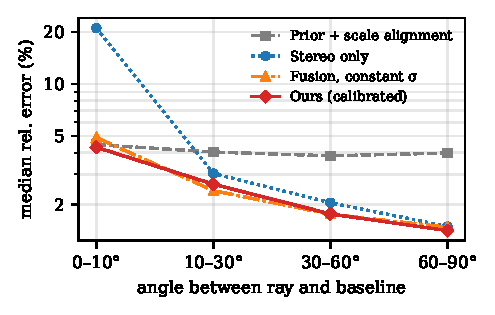
\includegraphics[width=\linewidth]{figures/error_vs_angle.pdf}
  \caption{Median relative error versus the angle between ray and baseline. Stereo diverges near the
  epipoles; the scale-aligned prior is flat; fusion follows the lower envelope.}
  \label{fig:angle}
\end{figure}

\Cref{tab:main,fig:angle} show the expected structure. Stereo alone is accurate orthogonal to the
baseline (1.49\% at 60--90$^\circ$) but useless near the epipoles (21\%). The prior is uniformly
mediocre, 6.95\% before and 3.94\% after scale alignment. Our fusion follows the lower envelope of the
two, reducing the median error of the raw prior from 6.95\% to 1.61\% overall while remaining
calibrated (0.71 of errors within $1\sigma$). Scale alignment matters: without it the error near the
epipoles rises from 4.30\% to 6.51\%. Evaluating $\U$ at the stereo depth is equivalent once the
precision is calibrated. The uncalibrated closed form ($\sigma_\theta=0.5$\,px) is as accurate overall
but badly calibrated (NLL $-1.36$ vs.\ $-2.16$), which motivates \cref{eq:calibration}: on this
benchmark, the implied matching precision varies by $6\times$ with the angle to the baseline.

\paragraph{An honest negative result.}
With its scale fitted on the same calibration rays, the geometry-blind \emph{confidence} baseline is as
accurate as ours in-distribution (1.60\% vs.\ 1.61\%) and has a slightly better NLL. The match
confidence already collapses near the epipoles, because all hypotheses project to nearly the same
pixel, so it implicitly encodes much of the observability. The same holds when transferring the
calibration to other baselines and resolutions (\cref{tab:transfer}): all calibrated fusion variants
are within 0.1 percentage points of each other. The closed form therefore does \emph{not}
improve accuracy over a well-calibrated confidence in the absence of pose error on this benchmark.

\begin{table*}[t]
  \centering
  \small
  \begin{tabular}{l cccccccc}
\toprule
 & \multicolumn{2}{c}{$b{=}2$\,m} & \multicolumn{2}{c}{$b{=}8$\,m} & \multicolumn{2}{c}{128$\times$256} & \multicolumn{2}{c}{512$\times$1024} \\
\cmidrule(lr){2-3}\cmidrule(lr){4-5}\cmidrule(lr){6-7}\cmidrule(lr){8-9}
Method & Med.\,(\%) & NLL & Med.\,(\%) & NLL & Med.\,(\%) & NLL & Med.\,(\%) & NLL \\
\midrule
Prior + scale alignment & 3.92 & -1.39 & 3.91 & -1.39 & 3.99 & -1.37 & 3.97 & -1.39 \\
Stereo only & 1.65 & 2.02 & 2.16 & 133.00 & 2.21 & 5.59 & 1.49 & 75.30 \\
Fusion, constant $\sigma_s$ & 1.57 & -2.25 & 1.82 & -1.87 & 1.94 & -2.03 & 1.46 & -2.18 \\
Fusion, confidence $\sigma_s$ & 1.52 & -2.32 & 1.81 & -1.92 & 1.89 & -2.10 & 1.41 & -2.22 \\
Ours (calibrated) & 1.51 & -2.29 & 1.82 & -1.89 & 1.97 & -2.03 & 1.38 & -2.00 \\
\bottomrule
\end{tabular}
  \caption{\textbf{Transfer without recalibration}: all methods are calibrated at $b=4$\,m and
  $256\times512$, and evaluated at other baselines and resolutions (5 scenes; 3 at $512\times1024$).}
  \label{tab:transfer}
  \label{sec:transfer}
\end{table*}

\subsection{Where geometry matters: relative-pose error}
\label{sec:pose}

\begin{table*}[t]
  \centering
  \small
  \begin{tabular}{l ccccccccc}
\toprule
 & \multicolumn{3}{c}{0.1$^\circ$/2cm} & \multicolumn{3}{c}{0.3$^\circ$/5cm} & \multicolumn{3}{c}{1$^\circ$/10cm} \\
\cmidrule(lr){2-4}\cmidrule(lr){5-7}\cmidrule(lr){8-10}
Method & Med. & Cal. & NLL & Med. & Cal. & NLL & Med. & Cal. & NLL \\
\midrule
Constant $\sigma_s$ & 1.77 & 0.70 & -2.08 & 2.34 & 0.59 & -1.70 & 3.99 & 0.44 & -0.50 \\
Constant $\sigma_s$, refit & 1.79 & 0.73 & -2.09 & 2.41 & 0.71 & -1.83 & 6.77 & 0.44 & -0.77 \\
Confidence $\sigma_s$ & \textbf{1.73} & 0.70 & -2.13 & 2.30 & 0.60 & -1.79 & 3.93 & 0.46 & -0.68 \\
Confidence $\sigma_s$, refit & 1.74 & 0.72 & \textbf{-2.13} & 2.36 & 0.71 & -1.87 & 6.52 & 0.44 & -0.82 \\
Ours w/o pose term & 1.74 & \textbf{0.69} & -2.08 & \textbf{2.26} & 0.60 & -1.78 & 3.86 & 0.46 & -0.68 \\
Ours & 1.75 & 0.71 & -2.09 & 2.28 & \textbf{0.70} & \textbf{-1.89} & \textbf{3.39} & \textbf{0.67} & \textbf{-1.54} \\
\bottomrule
\end{tabular}
  \caption{\textbf{Relative-pose error.} The partner pose given to all methods is perturbed by
  rotation/translation noise with the stated per-axis standard deviations; images are rendered with the
  true poses. ``refit'': geometry-blind baselines recalibrated on calibration scenes with the same pose
  noise. Ours uses the known noise level in the closed-form pose term (\cref{eq:sigma}) and is
  \emph{not} recalibrated. 8 test scenes.}
  \label{tab:pose}
\end{table*}

Poses from GNSS/IMU or SfM are never exact, and their error affects rays very differently: by
\cref{eq:sigma}, a translation error moves the depth by $\delta/\sin\gamma$, which is negligible
for close points orthogonal to the baseline and dominant for distant points and near the epipoles. Match
confidence cannot see this, because the cost curve can be sharply peaked at a wrong depth.
\Cref{tab:pose} injects pose errors into the partner pose. For small errors ($0.1^\circ$, 2\,cm) all methods are
equivalent. At $0.3^\circ$/5\,cm the geometry-blind uncertainties become over-confident (0.59--0.60 of
errors within $1\sigma$), while ours stays calibrated (0.70) and has the best NLL, at equal accuracy.
At $1^\circ$/10\,cm the pose term changes the result: ours reduces the median error from 3.93\% (best
baseline) to 3.39\%, raises the in-$1\sigma$ fraction from 0.46 to 0.67, and improves the NLL from
$-0.82$ to $-1.54$. Refitting the geometry-blind baselines under the same pose noise restores
calibration at moderate noise. At large noise, however, it inflates $\sigma_s$ uniformly, so no ray
remains reliable enough for scale alignment and the result degrades towards the unaligned prior
(6.5--6.8\%). Ours keeps rays orthogonal to the baseline at close range trustworthy, because there the pose
term is small. The pose term assumes the noise level is known; in practice it would come from the
SfM covariance or the GNSS/IMU specification.

\paragraph{Partners with different baselines.}
With two partners at $+2$\,m and $-8$\,m, all calibrated variants reach the same accuracy
(1.19--1.21\%) and similar calibration, \ie we observe no benefit of geometric weighting across
partners on this benchmark.

\subsection{Capture effects}
\label{sec:capture}

\begin{table}[t]
  \centering
  \footnotesize
  \setlength{\tabcolsep}{1.8pt}
  \begin{tabular}{l ccccc}
\toprule
Method & clean & exposure & noise & moving cars & all \\
\midrule
Confidence $\sigma_s$, L1 & \textbf{1.59} & 5.69 & 2.26 & \textbf{1.62} & 9.07 \\
Confidence $\sigma_s$, ZNCC & 5.29 & 5.42 & 6.50 & 5.32 & 6.72 \\
Ours, L1 & 1.60 & 5.96 & \textbf{2.24} & 1.63 & 8.51 \\
Ours, ZNCC, w/o outlier gate & 3.06 & 3.06 & 3.95 & 3.09 & 4.57 \\
Ours, ZNCC & 2.80 & \textbf{2.88} & 3.92 & 2.82 & \textbf{4.56} \\
\bottomrule
\end{tabular}
  \caption{\textbf{Capture effects} (median relative error, \%, 8 scenes): partner exposure change
  (gain 0.6, bias 0.15), sensor noise ($\sigma=0.03$), half of the parked cars moved by 3\,m between
  captures, and all three combined. Each cost function has its own calibration.}
  \label{tab:capture}
\end{table}

\Cref{tab:capture} varies the capture conditions. Two findings stand out. First, the cost
function matters: L1 is best for clean images and under sensor noise, while ZNCC is far more robust to
an exposure change between captures (2.88\% vs.\ 5.96\%) and in the combined setting (4.56\%
vs.\ 8.51\%). Second, with ZNCC the geometry-blind confidence baseline breaks down (5.29\% vs.\ 2.80\%
on clean data, 6.72\% vs.\ 4.56\% combined). Its success with L1 rests on the L1 confidence happening
to encode the epipolar degeneracy, which does not hold for every cost. The closed form does not depend
on such a coincidence. The outlier gate gives a modest gain on clean data and with moving cars
(3.06\%$\to$2.80\% and 3.09\%$\to$2.82\%), and none in the combined setting.

\subsection{Calibrating from a noisy city teacher}
\label{sec:teacher_cal}

\begin{table}[t]
  \centering
  \footnotesize
  \setlength{\tabcolsep}{3pt}
  \begin{tabular}{l c ccc}
\toprule
Calibration data & $\kappa$ & Med.\ rel.\ (\%) & Cal.\ $1\sigma$ & NLL \\
\midrule
Ground truth (oracle) & 0.38 & 1.61 & 0.71 & -2.16 \\
\midrule
Teacher, naive & 0.40 & 1.62 & 0.73 & -2.15 \\
Teacher, $\geq$2 views & 0.35 & 1.62 & 0.73 & -2.16 \\
Teacher, covariance-aware (ours) & 0.30 & 1.61 & 0.73 & -2.17 \\
\bottomrule
\end{tabular}
  \caption{\textbf{Calibration data.} The precision model of \cref{eq:calibration} is fitted on depth
  from a simulated city teacher (7 panoramas per street, lateral offsets, points displaced by draws
  from their own triangulation covariance, 0.5\,px matching at 2048\,px width) instead of ground truth.
  Evaluation as in \cref{tab:main}.}
  \label{tab:teacher}
\end{table}

Fitting the calibration on noisy teacher depth instead of ground truth costs nothing
measurable (\cref{tab:teacher}): all variants reach 1.61--1.62\% with calibrated uncertainties. Treating
the teacher as exact inflates the fitted scales slightly, as expected, because teacher error is
absorbed into the matching precision. Adding the teacher covariance in quadrature removes this
inflation. Downstream, however, the difference is negligible here, because the simulated teacher is
about $8\times$ more precise than the $512$\,px stereo it calibrates. Covariance-aware calibration
should matter only for teachers of comparable precision; we have not tested that regime.
